% =====================================================================
%  CXR Nodule Detection — bản thảo bài báo
%
%  Biên dịch:  pdflatex main.tex && bibtex main && pdflatex main.tex x2
%
%  ĐỔI ĐỊNH DẠNG KHI NỘP:
%    MICCAI workshop : \documentclass{llncs}      (cần llncs.cls)
%    IEEE EMBC       : \documentclass[conference]{IEEEtran}
%    Tạp chí Q2      : theo mẫu của tạp chí
%  Thân bài không phụ thuộc lớp tài liệu nên đổi được mà không phải viết lại.
%
%  MỌI CHỖ \todo{} LÀ VIỆC CHƯA XONG. Đừng nộp khi còn \todo{}.
%  Đặc biệt: tất cả trích dẫn đang là CHỖ TRỐNG. Xem paper/README_PAPER.md.
% =====================================================================
\documentclass[11pt,a4paper]{article}

\usepackage[utf8]{inputenc}
\usepackage[T1]{fontenc}
\usepackage{amsmath,amssymb}
\usepackage{booktabs}
\usepackage{graphicx}
\usepackage{xcolor}
\usepackage[margin=2.5cm]{geometry}
\usepackage{hyperref}
\hypersetup{colorlinks=true,linkcolor=blue,citecolor=blue,urlcolor=blue}

% Chỗ trống hiện rõ màu đỏ để không nộp nhầm khi còn thiếu.
\newcommand{\todo}[1]{\textcolor{red}{\textbf{[TODO: #1]}}}
\newcommand{\pending}[1]{\textcolor{orange}{\textbf{[PENDING: #1]}}}

\title{\textbf{Subtlety-Stratified Evaluation of Nodule Detection in Chest
Radiographs: Aggregate Gains Replicate, Their Stratified Attribution Does Not}}

% TÊN TÁC GIẢ VIẾT BẰNG MACRO, ĐỪNG THAY BẰNG CHỮ VIỆT TRỰC TIẾP.
% pdflatex + inputenc KHÔNG đọc được ầ (U+1EA7) và ị (U+1ECB): nó không báo
% lỗi dừng mà lặng lẽ BỎ MẤT chữ — "Trần Thị" in ra thành "Trn Th".
% Viết sai tên người là lỗi không được phép. Nếu sau này đổi sang XeLaTeX
% hoặc LuaLaTeX thì mới thay bằng chữ Việt trực tiếp được.
\author{B\`ui V\u{a}n X\'ia \and Tr\`{\^a}n Th\d{\i} Qu\`ynh Nga \\[2pt]
\normalsize Independent Researcher, Vietnam \\
\normalsize \texttt{buivanxia10@gmail.com}}
\date{}

\begin{document}
\maketitle

% =====================================================================
\begin{abstract}
\noindent
Pulmonary nodule detection on chest radiographs is usually summarised by one
aggregate figure such as the competition performance metric (CPM). Because easy
nodules outnumber hard ones, that figure is dominated by cases a radiologist
would already have seen. We evaluate detection on JSRT (247 images, 154 nodules)
stratified by the five-level radiologist subtlety rating, attaching an
image-level cluster bootstrap interval to every figure.

Bone suppression, proposed but not tested by earlier stratified work on this
dataset, raises aggregate CPM reproducibly: $+2.9$ points
$[+0.7, +5.1]$ across five seeds under ten-fold, and $+4.3$ $[+0.7, +8.6]$ under
leave-one-out. \emph{Where} that gain sits does not replicate --- ten-fold
attributes it to the second-easiest stratum, leave-one-out to the second-hardest
--- and we report this rather than resolve it, because at 12--50 nodules per
stratum a per-stratum estimate cannot carry a mechanistic claim.

Establishing even the aggregate effect required separating training from
sampling uncertainty, which are routinely conflated: a single-run bootstrap
gives $[-0.9, +6.3]$ and hides the effect, because roughly four CPM points of
run-to-run spread from random initialisation are absorbed into what that
interval presents as sampling error.

Detection of the most subtle stratum stays between 0\% and 8\% under every
configuration and both protocols, and does not move even under a manipulation
that halves overall performance. Applied unchanged to 1{,}426 VinDr-CXR images,
the detector reaches 16.5\% $[14.7, 18.3]$ against 43.3\% internally, under a
match tolerance more generous than the internal one.

We claim no novelty for stratified evaluation or for the frozen-backbone
observation, both reported previously.

\medskip
\noindent\textbf{Keywords:} chest radiography, nodule detection, subtlety
stratification, FROC analysis, bootstrap confidence intervals, reproducibility
\end{abstract}

% =====================================================================
\section{Introduction}

A pulmonary nodule that is plainly visible on a chest radiograph is not the
case that needs a second reader. The cases that matter are the ones a
radiologist may miss: small, low-contrast lesions, or lesions overlapped by
ribs and clavicles. Retrospective reviews of missed lung cancer on chest
radiographs consistently find that the lesion was visible in hindsight ---
Quekel~et~al.~\cite{quekel1999missrate} report that 19\% of lung cancers were
missed on a radiograph where the lesion could be seen retrospectively, with
superimposed bone and vascular structures the dominant cause. That is precisely
the population a detection system should target, and precisely the population
bone suppression is meant to help.

Reported performance rarely reflects this. The standard summary is the
competition performance metric (CPM), the mean sensitivity across a fixed set
of false-positive rates. CPM is computed over all nodules at once. When the
easy nodules outnumber the hard ones, as they do in every public dataset we are
aware of, CPM is largely a measure of performance on cases of limited clinical
interest. A system can post a respectable CPM while detecting almost nothing in
the subtle stratum.

The JSRT dataset is unusual in permitting a direct test, because each nodule
carries a subtlety rating from 1 (extremely subtle) to 5 (obvious) assigned by
three independent chest radiologists. That scale is not merely an expert
impression: in the database's own observer study, the mean confidence score of
20 radiologists reading the same cases correlates with the assigned subtlety
degree at $r = 0.999$~\cite{shiraishi2000jsrt}. The stratification axis we use
is therefore anchored to measured human detection difficulty, which is what
makes a per-stratum result clinically interpretable rather than an arbitrary
partition. This paper uses that rating in two ways. We report
sensitivity per stratum rather than in aggregate, and, more importantly, we
attach a confidence interval to every stratified figure.

The second step turns out to matter more than the first. Stratifying 154
nodules into five levels leaves 25 nodules in the hardest stratum and 12 in the
easiest. At those counts a single nodule changing state moves the reported
sensitivity by four to eight percentage points. Differences of that size are
routinely reported as improvements. We show they should not be.

Our contributions:

\begin{enumerate}
  \item A subtlety-stratified comparison of detection configurations on JSRT in
        which every figure, aggregate and per-stratum, carries a bootstrap
        confidence interval.
  \item A procedure that separates training uncertainty from sampling
        uncertainty --- averaging over seeds, then applying an image-level
        cluster bootstrap to that average. We show that reporting either alone
        is misleading in both directions, and that on this dataset the
        single-run interval conceals a real effect.
  \item A measurement of run-to-run variability due to random initialisation,
        which we find comparable in magnitude to the architectural effects
        under study.
  \item Evidence that the most subtle stratum resists every configuration
        tested, and does not move even under a manipulation that halves
        aggregate performance.
  \item A direct test of the standard explanation for why augmentation degrades
        a frozen-backbone detector, by partially unfreezing the backbone.
  \item External validation on VinDr-CXR with the match-tolerance difference
        measured and removed, so that the drop is attributed to generalisation
        rather than to a change of criterion.
\end{enumerate}

Every configuration we draw a conclusion from was run with a fixed seed and
its per-image scores retained, so all intervals in this paper can be recomputed
from the released scores without retraining. Two rows of Table~\ref{tab:loocv}
come from earlier runs that were neither seeded nor score-retaining; they are
labelled as such, and no claim rests on them.

We make no claim of priority. Horry~et~al.~\cite{horry2023fullres} analysed
JSRT by subtlety with a full-resolution encoder--decoder, observed the same
collapse on the lowest strata, and proposed the specific remedy we evaluate:
``Rib and bone suppression techniques \ldots could be expected to improve both
sensitivities of this algorithm and reduce false positive rates.'' They did not
evaluate it, reporting instead that the work was underway. This paper tests that
proposal. The improvement is real and replicates across two cross-validation
protocols; which difficulty stratum supplies it does not replicate, and the
stratum their analysis identified as the problem moves under neither.

% =====================================================================
\section{Related Work}

\paragraph{Nodule detection on chest radiographs.}
Automated nodule detection on chest radiographs is now dominated by deep
detectors and segmentation networks, benchmarked most visibly by the NODE21
challenge~\cite{sogancioglu2024node21}. Reported performance is almost always a
single aggregate figure --- a sensitivity at a chosen false-positive rate, or a
CPM --- computed over all nodules at once. Where a per-difficulty breakdown does
appear, as in Horry~et~al.~\cite{horry2023fullres}, it shows the aggregate
figure concealing near-total failure on the hardest cases.

\paragraph{Subtlety-stratified evaluation.}
Stratifying JSRT results by the subtlety rating is not new.
Horry~et~al.~\cite{horry2023fullres} evaluate a full-resolution
encoder--decoder per subtlety level and observe the same collapse on the lowest
levels that we observe here. That work proposes bone suppression as a plausible
remedy but does not evaluate it. Our study should be read as a test of that
proposal rather than as an independent idea.

That paper also illustrates, transparently and in its own words, why the
stratification matters for how results are read. Its strongest external
generalisation figure --- 76.7\% sensitivity at 7.6 false positives per image
--- was obtained ``when very subtle and extremely subtle nodules were excluded
from the JSRT training data''~\cite{horry2023fullres}, and the authors record
that their best configuration excluded those categories. We note this not as a
criticism, since it is stated plainly in the source, but because it makes the
point concrete: a headline detection figure is conditional on which difficulty
strata are in scope, and the two hardest strata are the ones most often out of
it.

\paragraph{Bone suppression.}
Suppressing rib and clavicle shadows is an established pre-processing step.
Early learned approaches trained autoencoders and convolutional networks to
regress the soft-tissue image~\cite{gusarev2017bonesup}, and recent generative
models reconstruct bone-free radiographs with high fidelity ---
Ibrahim~et~al.~\cite{ibrahim2025bonesup} report SSIM $0.99$ on JSRT. That
literature is evaluated on image-reconstruction quality, not on whether
suppression improves lesion \emph{detection}, and never per subtlety stratum.
The gap we address is the downstream one.

\paragraph{Foundation models for medical imaging.}
RAD-DINO~\cite{perezgarcia2024raddino} is a self-supervised vision transformer
trained on a large corpus of chest radiographs. One detail matters for
interpreting our results. RAD-DINO as proposed was trained on 838k images, of
which 90k come from a private cohort; the authors additionally trained a
public-data-only variant for release. The \texttt{microsoft/rad-dino} checkpoint
we use is that public variant, whose constituent datasets sum to roughly 748k
images. We therefore do not attribute the 838k figure to the model we actually
ran.
Muthyala~et~al.~\cite{muthyala2026frozen} probe five frozen vision transformers,
RAD-DINO among them, and show that small-lesion signal is discarded at the
global-aggregation step while remaining recoverable from patch tokens. Their
evidence is classification AUC on NIH-CXR14, MIMIC-CXR, Emory-CXR and
ChestX-Det10; ours is detection on JSRT stratified by subtlety. The two are
complementary, and we treat their result as the prior finding rather than our
own discovery. We note that our decoder consumes patch tokens rather than the
class token --- the configuration their analysis identifies as retaining the
signal --- so our persistent failure on the most subtle stratum is not
explained by global aggregation alone.

\paragraph{Benchmarks and contamination.}
JSRT is included in the training data of NODE21~\cite{sogancioglu2024node21}, the current
standard benchmark for nodule detection on chest radiographs. Results on JSRT
therefore cannot be compared directly against models that have seen NODE21
training data, and we make no such comparison.

% =====================================================================
\section{Materials and Methods}

\subsection{Data}

\paragraph{JSRT.}
The JSRT dataset~\cite{shiraishi2000jsrt} contains 247 posteroanterior chest
radiographs collected from 14 medical centres: 154 with a single pulmonary
nodule confirmed by CT, and 93 without. Films were digitised at
$2048 \times 2048$ with 0.175\,mm pixels. Each nodule carries a subtlety rating
from 1 to 5 assigned by three chest radiologists, reflecting nodule size,
density and occlusion by overlying structures. The distribution is uneven --- 25, 29, 50, 38 and 12 nodules at
levels 1 through 5 --- and the two extreme strata are small enough that we
interpret differences there with corresponding caution. Every positive case
carries exactly one nodule; diameters range from 5 to 60\,mm with a median of
15\,mm. Images were resampled
to $512 \times 512$ and contrast-limited adaptive histogram equalisation was
applied (clip limit 2.0, $8 \times 8$ grid).

\paragraph{NIH ChestX-ray14.}
112{,}120 images from ChestX-ray14~\cite{wang2017chestxray} were used to
pre-train the ResNet-34 backbone. Labels in this
dataset are mined automatically from radiology reports and are known to be
noisy~\cite{oakdenrayner2020exploring}; we use it only for representation
learning and never for evaluation.

\paragraph{Bone-shadow pairs.}
241 paired radiographs with and without bone shadow were used to train the
suppression network described below. The originals are the JSRT
images~\cite{shiraishi2000jsrt}; the bone-suppressed counterparts are the
BSE-JSRT set produced by Juh\'asz~et~al.~\cite{juhasz2010bse}. JSRT contains 247
images and the bone-suppressed release covers 241 of them. We obtained the pair
set through a Kaggle redistribution, which is an access point rather than a
source.

\subsection{Detection Framework}

We treat detection as heatmap regression. Each nodule centre generates a
Gaussian target ($\sigma = 8$ px) on a stride-4 output grid; the value at the
rounded centre pixel is forced to exactly 1.0, without which the positive class
is never represented exactly and the network fails to train. Predictions are
decoded by non-maximum suppression with a minimum peak separation of 10 px.

Training minimises a focal mean-squared-error loss. Gradients are clipped to
norm 5.0. \textbf{Mixed precision is disabled}: with automatic mixed precision
enabled the loss underflowed to exactly zero and the network did not learn at
all. We note this because it cost considerable debugging time and is not, to
our knowledge, documented for this class of loss.

\subsection{Configurations Compared}
\label{sec:configs}

\begin{description}
  \item[Baseline.] ResNet-34 encoder pre-trained on NIH ChestX-ray14, single
        grayscale input channel.
  \item[Bone suppression + attention.] The same encoder with a second input
        channel carrying a bone-suppressed image produced by a U-Net trained on
        the paired data, plus CBAM attention blocks~\cite{woo2018cbam}.
  \item[Foundation model.] The public \texttt{microsoft/rad-dino} checkpoint
        (87M parameters as reported; 86.6M in the released weights) with all
        weights frozen, used as a feature extractor. Input channels are $[\text{original}, \text{bone-suppressed},
        \text{original}]$. A lightweight convolutional decoder is trained on the
        extracted features.
\end{description}

\subsection{Evaluation Protocol}

We report free-response ROC (FROC) analysis. A detection counts as a hit when
its peak falls within 15\,mm of a true nodule centre; each nodule may be matched
at most once, and unmatched peaks are false positives. CPM is the mean
sensitivity at 0.125, 0.25, 0.5, 1.0, 2.0 and 4.0 false positives per image.

Stratified sensitivity uses \emph{the same operating thresholds} as the
aggregate FROC curve. This point is easy to get wrong: computing stratified
sensitivity by counting all detections without applying the FROC threshold
inflates the figures substantially and destroys their monotonicity with respect
to subtlety. We made this error twice during development before catching it.

The primary protocol is leave-one-out cross-validation, which maximises
training data on a small dataset. Ten-fold cross-validation is used for the
ablation study, where the number of configurations makes leave-one-out
prohibitive. Folds are split \emph{by image}, so that all augmented variants of
an image fall on the same side of the split; splitting by variant leaks
training data into the test fold.

\subsection{Uncertainty Quantification}
\label{sec:bootstrap}

Every figure we report carries a 95\% bias-corrected and accelerated (BCa)
bootstrap confidence interval over $B = 2000$ resamples with a fixed resampling
seed, so the intervals are exactly reproducible; different resampling seeds move
interval endpoints by a few tenths of a point. Three design choices
matter, and getting any of them wrong produces intervals that are too narrow.

\paragraph{Resample images, not nodules.}
The FROC operating threshold is defined by a false-positive count \emph{per
image}. Resampling individual nodules leaves the number of images undefined and
detaches false positives from the images that produced them, which makes the
threshold meaningless. We therefore resample images with replacement; a
selected image contributes all of its nodules and all of its false positives.

\paragraph{Recompute the threshold inside each resample.}
Holding the original-sample threshold fixed ignores the uncertainty in
estimating that threshold. In each resample we therefore recompute the threshold
from that resample's own false-positive scores. We measured what this costs by
running both variants on identical resamples, differing only in whether the
threshold is recomputed: fixing it narrows intervals by 2.9\% on average and by
up to 11.8\% at individual operating points. The effect is real but modest, and
we report the magnitude rather than assert that it is large --- on this dataset
the choice does not change any conclusion, and the larger distortion by far is
the conflation described in Section~\ref{sec:twonoise}.

\paragraph{Pair the comparison.}
When comparing two configurations we resample the same image indices for both
and form the interval on the \emph{difference}. Both configurations are
evaluated on the same 247 images, so most of the variance is shared and
cancels. An unpaired comparison discards this and produces an interval much
wider than necessary.

Because the stratified comparisons involve five strata at several operating
points, we make no multiplicity correction and treat those results as
exploratory.

Two limitations of the procedure should be stated. The BCa acceleration is
estimated by a jackknife over images, which assumes the statistic behaves
smoothly under deletion; the threshold recomputation makes it only piecewise
smooth, so the interval endpoints carry some approximation error beyond Monte
Carlo noise. And the seed-averaged estimator of Section~\ref{sec:twonoise}
bootstraps images around an average of five runs, which propagates sampling
uncertainty but not the uncertainty of having estimated that average from five
seeds rather than many.

% =====================================================================
\section{Results}

\subsection{Aggregate Performance}

Table~\ref{tab:loocv} reports leave-one-out CPM. Aggregate performance
increases across the three configurations.

\begin{table}[t]
\centering
\caption{Leave-one-out cross-validation on JSRT. The two RAD-DINO rows are
seeded runs with per-image scores retained, so intervals are computable; the
ResNet-34 rows are earlier single runs with no fixed seed and no retained
scores, and establish nothing on their own.}
\label{tab:loocv}
\begin{tabular}{llc}
\toprule
Configuration & Architecture & CPM (\%) [95\% CI] \\
\midrule
\multicolumn{3}{l}{\emph{Seeded, intervals computable:}} \\
3-channel        & RAD-DINO (frozen)          & 40.3 $[34.0, 48.0]$ \\
+ bone suppression & RAD-DINO (frozen) + U-Net & 44.6 $[37.7, 51.3]$ \\
\midrule
\multicolumn{3}{l}{\emph{Earlier single unseeded runs, no interval:}} \\
Baseline                       & ResNet-34                & 29.5 \\
+ bone suppression + attention & ResNet-34 + U-Net + CBAM & 34.2 \\
\bottomrule
\end{tabular}
\end{table}

Under leave-one-out, bone suppression gives $+4.3$ CPM points
$[+0.7, +8.6]$, an interval excluding zero and consistent in sign and rough
magnitude with the $+2.9$ $[+0.7, +5.1]$ obtained from five seeds under ten-fold
(Section~\ref{sec:twonoise}). The aggregate effect replicates across protocols.

\begin{figure}[t]
\centering
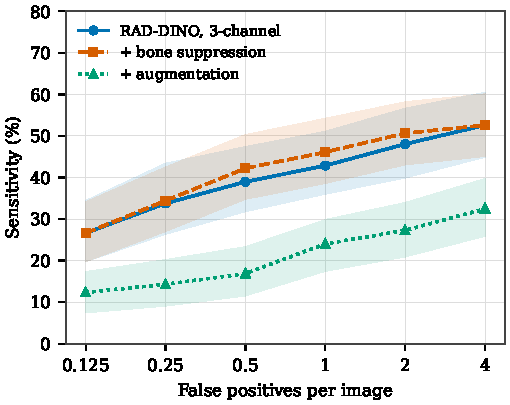
\includegraphics{fig/fig_froc.pdf}
\caption{FROC curves for three RAD-DINO configurations (ten-fold). Shaded bands
are 95\% image-level bootstrap intervals. The bone-suppressed and 3-channel
curves overlap across most of the range; the augmented configuration is
separated from both throughout. Line style and marker encode configuration in
addition to colour, so the figure survives greyscale printing.}
\label{fig:froc}
\end{figure}

\subsection{Stratification Reverses the Ordering}

Table~\ref{tab:strat} tells a different story. The configuration with bone
suppression and attention improves the two hardest strata over baseline
(0.0\%~$\rightarrow$~8.0\% and 6.9\%~$\rightarrow$~20.7\%) while
\emph{losing} ground on the two easiest (68.4\%~$\rightarrow$~57.9\% and
83.3\%~$\rightarrow$~58.3\%). Aggregate CPM, which rose from 29.5 to 34.2,
conceals this trade entirely.

\begin{table}[t]
\centering
\caption{Sensitivity by subtlety level at 1.0 false positive per image,
from the same earlier single unseeded runs as Table~\ref{tab:loocv} and subject
to the same caveat. Level 1 is the most subtle. Note the small denominators: at
$n=12$ one nodule is 8.3 percentage points.}
\label{tab:strat}
\begin{tabular}{lcccc}
\toprule
Subtlety level & $n$ & Baseline & ResNet34+U-Net+CBAM & RAD-DINO+U-Net \\
\midrule
1 --- extremely subtle & 25 &  0.0 &  8.0 &  4.0 \\
2 --- very subtle      & 29 &  6.9 & 20.7 & 27.6 \\
3 --- moderate         & 50 & 20.0 & 32.0 & 48.0 \\
4 --- fairly obvious   & 38 & 68.4 & 57.9 & 73.7 \\
5 --- obvious          & 12 & 83.3 & 58.3 & 75.0 \\
\bottomrule
\end{tabular}
\end{table}

\begin{figure}[t]
\centering
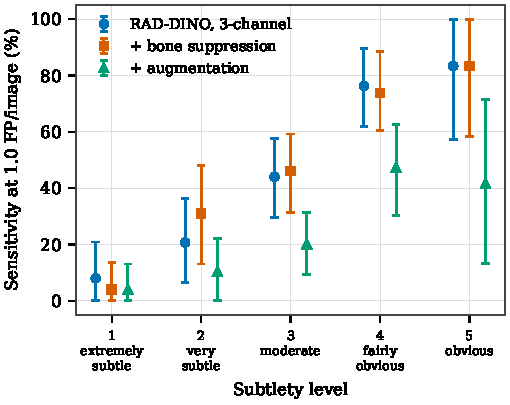
\includegraphics{fig/fig_strat.pdf}
\caption{Sensitivity at 1.0 FP/image by subtlety level, with 95\% image-level
bootstrap intervals. The intervals are wide at every level and overlap almost
everywhere --- which is the point: at 12--50 nodules per stratum, differences of
the size usually reported as improvements cannot be resolved.}
\label{fig:strat}
\end{figure}

We stress what the level-1 column does \emph{not} show. The difference between
8.0\% and 4.0\% is one nodule out of 25. It is not evidence that either
configuration is better, and we do not interpret it as such.

\subsection{Run-to-Run Variability}
\label{sec:noise}

Re-running a configuration with an identical seed and configuration file
produced a CPM of 40.5\% where 36.5\% had been recorded previously. The cause
was that the random seed governed the cross-validation split but was never
applied to the weight initialisation of the detection head. Across five seeds
the 3-channel configuration scores $40.4 \pm 1.0$ and the bone-suppressed
configuration $43.3 \pm 1.4$ CPM.

This matters for how the remaining results must be read. A four-point spread
from initialisation alone is comparable to the effect sizes commonly reported
as improvements on this benchmark, so a single training run cannot establish
one.

\subsection{Separating Training Noise from Sampling Noise}
\label{sec:twonoise}

Two distinct uncertainties act on these numbers, and conflating them leads to
error in both directions.

Training uncertainty asks whether a re-run reproduces the result; it is
measured by repeating the experiment across seeds. Sampling uncertainty asks
whether the result would hold on a different set of 247 images; it is measured
by the image-level bootstrap of Section~\ref{sec:bootstrap}. Reporting either
alone is misleading. A bootstrap interval from one training run absorbs
initialisation noise into what it presents as sampling uncertainty, and is
correspondingly too wide. A standard deviation across seeds is computed on a
single fixed image set and says nothing about generalisation.

We therefore take as the primary estimator the \emph{seed-averaged difference},
and bootstrap images around it: within each resample the same image indices are
applied to all ten runs, the per-seed difference is computed, and those
differences are averaged. This averages away training noise while preserving
sampling uncertainty.

Table~\ref{tab:bone} applies this to the bone-suppression contrast. The
difference is $+2.9$ CPM points with a 95\% interval of $[+0.7, +5.1]$, and it
is positive in all five seeds individually.

\begin{table}[t]
\centering
\caption{Bone suppression, five seeds, ten-fold cross-validation. Per-seed
differences are consistently positive. The pooled interval is an image-level
bootstrap ($B = 2000$) on the seed-averaged difference.}
\label{tab:bone}
\begin{tabular}{lccc}
\toprule
Seed & 3-channel & + bone supp. & $\Delta$ \\
\midrule
0 & 40.5 & 42.1 & $+1.6$ \\
1 & 41.9 & 44.8 & $+2.9$ \\
2 & 39.3 & 42.0 & $+2.7$ \\
3 & 40.0 & 42.9 & $+2.8$ \\
4 & 40.2 & 44.7 & $+4.5$ \\
\midrule
Mean $\pm$ SD & $40.4 \pm 1.0$ & $43.3 \pm 1.4$ & $+2.9 \pm 1.0$ \\
\midrule
\multicolumn{3}{l}{Pooled, image bootstrap [95\% CI]} & $+2.9$ $[+0.7, +5.1]$ \\
\bottomrule
\end{tabular}
\end{table}

Two points follow. First, the effect is real but small. A previously recorded
figure of $+7.9$ points for this contrast does not reproduce; the reproducible
effect is roughly $+2.9$, and the remainder is attributable to initialisation
noise in a single-run comparison. Second, a single-seed bootstrap on these same
data gives $+2.8$ with an interval of $[-0.9, +6.3]$, which contains zero. The
effect is not absent in that analysis --- it is obscured by training noise that
the pooled estimator removes.

\subsection{Where the Gain Actually Falls}
\label{sec:where}

Table~\ref{tab:bonestrat} decomposes the bone-suppression gain by subtlety.

\begin{table}[t]
\centering
\caption{Bone-suppression gain by subtlety level at 1.0 FP/image, seed-averaged
over five seeds with image-level bootstrap intervals.}
\label{tab:bonestrat}
\begin{tabular}{lcc}
\toprule
Subtlety level & $\Delta$ (points) & 95\% CI \\
\midrule
1 --- extremely subtle & $-0.8$ & $[-8.6, +7.5]$ \\
2 --- very subtle      & $+1.4$ & $[-5.8, +8.5]$ \\
3 --- moderate         & $+1.6$ & $[-4.5, +8.0]$ \\
4 --- fairly obvious   & $+6.3$ & $[+1.9, +11.4]$ \\
5 --- obvious          & $+10.0$ & $[-1.4, +20.0]$ \\
\bottomrule
\end{tabular}
\end{table}

\begin{figure}[t]
\centering
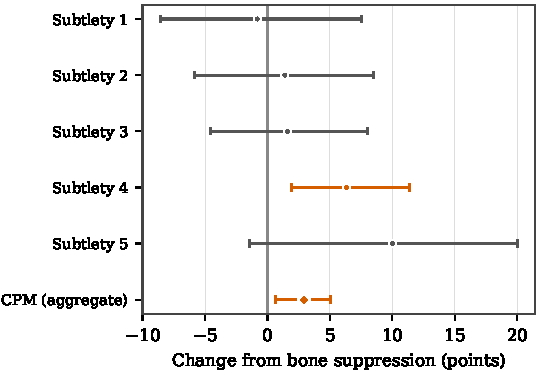
\includegraphics{fig/fig_forest.pdf}
\caption{Effect of bone suppression by subtlety level under ten-fold
cross-validation, averaged over five seeds, with 95\% image-level bootstrap
intervals; intervals excluding zero are drawn in colour. The aggregate gain is
real and replicates under leave-one-out, but this per-stratum pattern does not:
under leave-one-out the gain moves to level 2 and level 5 turns negative
(Table~\ref{tab:unstable}). Read the aggregate row as the finding and the
per-stratum rows as provisional.}
\label{fig:forest}
\end{figure}

The only stratum with an interval excluding zero is level 4, the second-easiest.
The point estimate on level 1 is negative. The aggregate gain of 2.9 CPM points
is therefore driven by nodules that were already fairly visible, and there is no
evidence of improvement where improvement would matter.

Figure~\ref{fig:forest} shows this at a glance. Bone suppression produces a
statistically defensible improvement in aggregate CPM. Reported as a single
number, that improvement would be taken as progress on nodule detection. Under
this protocol, stratifying it shows progress on the nodules a radiologist was
least likely to miss. Section~\ref{sec:unstable} shows that a second protocol
relocates the gain to a different stratum, so this particular attribution is
provisional; what is not provisional is that one aggregate number cannot tell
you which cases improved.

\subsection{Which Stratum Benefits Is Not Stable Across Protocols}
\label{sec:unstable}

The aggregate effect replicates. The stratified attribution does not.

\begin{table}[t]
\centering
\caption{Bone-suppression gain per subtlety level at 1.0 FP/image under two
protocols. Bold marks intervals excluding zero. The protocols agree on the
aggregate but disagree on which stratum carries it.}
\label{tab:unstable}
\begin{tabular}{lcc}
\toprule
Subtlety level & Ten-fold, 5 seeds pooled & Leave-one-out, 1 seed \\
\midrule
1 --- extremely subtle & $-0.8$ & $+0.0$ \\
2 --- very subtle      & $+1.4$ & $\mathbf{+17.2}$ $[+3.8, +31.0]$ \\
3 --- moderate         & $+1.6$ & $+4.0$ \\
4 --- fairly obvious   & $\mathbf{+6.3}$ $[+1.9, +11.4]$ & $+13.2$ $[0.0, +24.5]$ \\
5 --- obvious          & $+10.0$ & $-16.7$ \\
\midrule
Aggregate CPM & $\mathbf{+2.9}$ $[+0.7, +5.1]$ & $\mathbf{+4.3}$ $[+0.7, +8.6]$ \\
\bottomrule
\end{tabular}
\end{table}

Under ten-fold with seeds pooled, the only stratum clearing zero is level 4 and
level 5 gains 10 points; under leave-one-out with a single seed, level 2 clears
zero with a 17-point gain while level 5 \emph{loses} 17. Both analyses use the
same images, the same model and the same bone-suppression channel.

We take the pooled ten-fold estimate as the more reliable of the two, because it
averages over five seeds and Section~\ref{sec:noise} measured roughly four CPM
points of run-to-run spread that a single run cannot remove. But we do not think
the disagreement should be explained away. It is the paper's own thesis turned on
its own results: with 12 to 50 nodules per stratum, a per-stratum estimate is not
stable enough to support a claim about \emph{where} a method helps, even when the
aggregate effect it produces is solid. Readers --- ourselves included --- should
resist the temptation to build a mechanistic story on top of a stratified
pattern at this sample size.

What survives both protocols is narrower and, we think, more trustworthy: bone
suppression improves aggregate CPM by a few points, and level 1 moves in neither
analysis.

\subsection{One Contrast Does Survive: Augmentation Under a Frozen Backbone}
\label{sec:aug}

Not every difference is lost in noise. Table~\ref{tab:aug} reports the effect of
augmenting the training data while the backbone stays frozen. CPM falls by 22.1
points, with a 95\% interval of $[-28.2, -16.1]$, and every individual operating
point excludes zero. This effect is an order of magnitude larger than the
initialisation noise quantified in Section~\ref{sec:noise}, and we report it
without reservation.

\begin{table}[t]
\centering
\caption{Paired image-level bootstrap for the augmentation contrast (RAD-DINO
with frozen backbone, ten-fold, $B = 3000$). Augmentation uses eight variants
per image. $\Delta$ is with-augmentation minus without.}
\label{tab:aug}
\begin{tabular}{lccc}
\toprule
Metric & No aug. & + augmentation & $\Delta$ [95\% CI] \\
\midrule
CPM                     & 43.3 & 21.2 & $-22.1$ $[-28.2, -16.1]$ \\
Sens @ 1.0 FP/image     & 46.1 & 24.0 & $-22.1$ $[-30.4, -14.2]$ \\
\midrule
\multicolumn{4}{l}{\emph{By subtlety, at 1.0 FP/image:}} \\
Level 1 (most subtle)   &  4.0 &  4.0 & $+0.0$ $[-11.5, +11.5]$ \\
Level 3                 & 46.0 & 20.0 & $-26.0$ $[-39.2, -12.2]$ \\
Level 5 (obvious)       & 83.3 & 41.7 & $-41.7$ $[-71.4, -11.8]$ \\
\bottomrule
\end{tabular}
\end{table}

The stratified rows carry an observation we did not anticipate. The degradation
is monotonic in subtlety --- the clearest nodules lose the most --- and level 1
does not move at all. A manipulation severe enough to halve overall performance
leaves the hardest stratum exactly where it was, because at 4\% (one nodule of
25) there is essentially nothing left to lose. We return to this floor effect
in Section~\ref{sec:floor}.

\subsection{Unfreezing the Backbone Removes Most of the Penalty}
\label{sec:ft}

Section~\ref{sec:aug} established that augmentation costs 22 CPM points while the
backbone is frozen, and offered an explanation: a frozen backbone cannot adapt to
transformed inputs, so augmented images fall outside the distribution its
features were learned on. That explanation predicts something testable. If it is
right, allowing the backbone to adapt should remove the penalty.

We unfroze the last four transformer blocks of RAD-DINO (28.4M of the
checkpoint's 86.6M parameters) and repeated the contrast. Both arms use identical settings
--- four unfrozen blocks, 20 epochs, five folds, batch 2, seed 42 --- and differ
only in whether augmentation is applied.

\begin{table}[t]
\centering
\caption{The augmentation penalty under a frozen versus a partially fine-tuned
backbone. Within each row both arms share a protocol and differ only in
augmentation; the two rows use different protocols and so are compared
qualitatively.}
\label{tab:ft}
\begin{tabular}{lccc}
\toprule
Backbone & No aug. & + augmentation & $\Delta$ [95\% CI] \\
\midrule
Frozen (10-fold, 60 ep.)        & 43.3 & 21.2 & $-22.1$ $[-28.2, -16.1]$ \\
4 blocks unfrozen (5-fold, 20 ep.) & 42.2 & 39.1 & $\phantom{0}-3.1$ $[-8.5, +2.1]$ \\
\bottomrule
\end{tabular}
\end{table}

The penalty falls from 22.1 points to 3.1, and the interval on the fine-tuned
contrast contains zero. The two intervals do not overlap. The prediction holds:
most of the damage augmentation does to this system is attributable to the
backbone being unable to adapt, not to the augmentation itself.

Two caveats bound this conclusion. The fine-tuned runs use five folds and 20
epochs against the frozen runs' ten folds and 60, so comparing the two
\emph{differences} is a comparison across protocols rather than a single
controlled experiment; within each row the comparison is controlled. And the
fine-tuned arms are single runs, where Section~\ref{sec:noise} measured a
run-to-run spread of roughly four CPM points --- large enough to matter for a
difference of 3.1. The qualitative collapse from 22 points to near zero is far
outside that noise; the residual 3.1 is not.

Fine-tuning did not improve aggregate performance: 42.2\% $[35.3, 49.3]$ against
43.3\% for the frozen backbone with bone suppression. Its value here is
explanatory rather than practical.

\subsection{External Validation on VinDr-CXR}
\label{sec:external}

We applied the JSRT-trained detector, unchanged, to 1{,}426 VinDr-CXR
images~\cite{nguyen2022vindr} containing 1{,}795 annotated nodules --- eleven
times more nodules than JSRT provides, so the intervals here are narrow. The
decoder was trained on all of JSRT and never saw VinDr.

A hit on VinDr requires the predicted peak to fall inside an annotated box.
This is not the criterion used on JSRT, where a hit is a peak within 15\,mm of
the nodule centre, and the two are not interchangeable: 15\,mm corresponds to
21.4 px at our resolution, whereas the median VinDr box admits a tolerance of
only 7.6 px. The external criterion is roughly $2.8\times$ stricter, and a naive
comparison would charge that difference to the model.

We therefore swept a margin that dilates each box before matching
(Table~\ref{tab:margin}), which separates the two effects.

\begin{table}[t]
\centering
\caption{External validation on VinDr-CXR under increasing match tolerance. A
margin of 21 px makes the effective tolerance more generous than the 21.4 px
used on JSRT, so the last row removes the criterion difference entirely.}
\label{tab:margin}
\begin{tabular}{lccc}
\toprule
Box margin & Effective tolerance & CPM (\%) & Sens @ 1.0 FP (\%) \\
\midrule
0 px (strict) & $\approx$ 7.6 px  & 13.7 & 15.2 \\
7 px          & $\approx$ 14.6 px & 14.8 & 16.5 \\
14 px         & $\approx$ 21.6 px & 15.7 & 17.4 \\
21 px         & $\approx$ 28.6 px & 16.5 $[14.7, 18.3]$ & 18.1 $[16.0, 20.4]$ \\
\bottomrule
\end{tabular}
\end{table}

Relaxing the criterion from stricter-than-JSRT to more-generous-than-JSRT moves
CPM by 2.8 points, from 13.7\% to 16.5\%. The internal figure for the same
configuration is 43.3\%. The measurement difference therefore explains roughly a
tenth of the gap; the remaining $\approx26$ points are a genuine failure to
transfer.

We report this plainly because it bears on the paper's argument. A system whose
internal stratified analysis we have just spent several sections refining
detects fewer than one nodule in five on an external cohort at one false
positive per image. Internal cross-validation on 247 images, however carefully
its uncertainty is quantified, did not predict this.

Three differences between the cohorts bound the interpretation, and none of them
is small. VinDr's \texttt{Nodule/Mass} class merges nodules with masses by
definition, while JSRT is predominantly nodules --- median diameter 15\,mm, and
97\% at or below 30\,mm, though 4 of its 154 lesions exceed that --- so the
detection targets overlap but are not the same population. The VinDr labels we used come from three independent readers
merged by IoU rather than the five-reader consensus of the official test split,
which is available only through PhysioNet. And acquisition, population and
post-processing all differ. We present this as evidence that the system does not
transfer, not as a calibrated estimate of how well it would transfer to a cohort
matched to JSRT.

\subsection{The Most Subtle Stratum Resists Every Configuration}
\label{sec:floor}

Across every configuration tested, sensitivity on subtlety level 1 ranges from
0\% to 8\% --- between zero and two nodules out of 25. This includes the
RAD-DINO configuration. Scale of pre-training does not, by itself, solve the
hardest detection problem in this dataset.

Table~\ref{tab:aug} sharpens the point from the opposite direction. Level 1 is
not merely unresponsive to changes that \emph{help}; it is equally unresponsive
to a change that severely \emph{hurts}. Augmentation under a frozen backbone
costs 22 CPM points overall and 42 points on the most obvious nodules, yet
leaves level 1 unchanged. The stratum behaves as a floor that our methods
neither raise nor lower.

See Section~\ref{sec:external}.

% =====================================================================
\section{Discussion}

\paragraph{What stratification buys.}
The pattern is visible in Tables~\ref{tab:loocv} and~\ref{tab:strat} read
together. Aggregate CPM rises monotonically across the three configurations, and
on that evidence one would recommend the third. The stratified table shows the
second configuration trading easy-nodule sensitivity for hard-nodule sensitivity
--- a trade that may well be desirable clinically, and one that aggregate
reporting renders invisible in either direction. Those two tables are single
unseeded runs and we draw no inference from them; the same phenomenon appears in
the seeded experiments below, where it can be quantified.

\paragraph{What confidence intervals take away.}
Having argued that stratification reveals structure hidden by aggregation, we
must report that much of that structure is not statistically resolvable at this
sample size. With 25 nodules in the hardest stratum, the bootstrap interval on a
stratified sensitivity spans tens of percentage points. We consider reporting
these intervals a requirement rather than an option: a stratified analysis
without them invites precisely the over-interpretation that stratification was
meant to prevent.

The bone-suppression result shows that the requirement cuts both ways. Reported
from one run, its interval contains zero and the effect looks absent; pooled
over seeds, the effect is real. Wide intervals are not automatically evidence
of no effect --- they may be evidence that the wrong noise source was
measured.

\paragraph{Frozen backbones and augmentation.}
Augmenting the training data while the backbone remained frozen reduced CPM by
22.1 points $[-28.2, -16.1]$. The natural account --- that a frozen backbone
cannot adapt to transformed inputs, so augmented images fall outside the
distribution its features were learned on --- makes a falsifiable prediction, and
Section~\ref{sec:ft} tests it. Unfreezing four transformer blocks reduces the
penalty to 3.1 points with an interval containing zero. The explanation survives
the test.

We note that this is the kind of claim most often left as an untested aside in
this literature. It cost one additional experiment to check, and had the penalty
persisted under fine-tuning we would have had to withdraw the explanation
entirely.

\paragraph{The hardest stratum, and what the backbone's authors already knew.}
Our failure on subtlety level 1 is not an anomalous result from an unusual
pipeline. The RAD-DINO authors report in their own appendix that performance
degrades at reduced input resolution specifically for subtle findings such as
pneumothorax and chest drains, and conclude that high resolution is needed to
detect fine-grained signs~\cite{perezgarcia2024raddino}. Our finding is the
detection analogue of that limitation, measured on a graded difficulty scale:
the stratum that resists every configuration is exactly the one the backbone's
own developers flag as resolution-sensitive. Read together with
Muthyala~et~al.~\cite{muthyala2026frozen}, who locate the loss at the
global-aggregation step, the picture is consistent --- though neither
explanation is sufficient here, since our decoder already reads patch tokens at
the native grid.

\paragraph{Relation to prior findings.}
Our observation that frozen foundation features lose small-lesion signal
reproduces a result published independently~\cite{muthyala2026frozen}. We regard the
agreement of two independent studies as more informative than either alone, and
we claim no priority.

\paragraph{External validation.}
Section~\ref{sec:external} reports the external result: CPM falls from 43.3\%
internally to 16.5\% $[14.7, 18.3]$ on VinDr-CXR even under a match tolerance
more generous than the internal one. We note that the hit criterion on
VinDr-CXR~\cite{nguyen2022vindr} differs from that used on JSRT: VinDr annotations are bounding boxes
and DICOM pixel spacing varies across images, so a millimetre-based radius is
unreliable and we instead require the predicted peak to fall inside the
annotated box. CPM values on the two datasets are therefore \emph{not} directly
comparable, and we use the external results only as a qualitative indication of
generalisation.

% =====================================================================
\section{Limitations}

\begin{enumerate}
  \item \textbf{Small, single-source dataset.} 247 images from one institution,
        with 154 nodules. Every confidence interval in this paper is wide as a
        direct consequence, and the stratified intervals are very wide.
  \item \textbf{One nodule per image.} JSRT contains a single nodule per
        positive case, which does not reflect clinical reality.
  \item \textbf{Mostly frozen backbone.} The main configurations use the public
        RAD-DINO checkpoint purely as a feature extractor, so those results characterise frozen
        features and not the model's ceiling. The partial fine-tuning of
        Section~\ref{sec:ft} uses a shorter protocol (five folds, 20 epochs) and
        a single seed, so it supports a qualitative conclusion about the
        augmentation penalty but not a precise effect size.
  \item \textbf{Performance below published work.} Our absolute CPM values are
        lower than results reported by others on JSRT.
        Horry~et~al.~\cite{horry2023fullres} reach 85\% sensitivity at 8 false
        positives per image internally and 76.7\% at 7.6 externally --- the
        latter with the two hardest subtlety categories excluded from training,
        and at a false-positive rate roughly twice the highest we report. We
        retained every stratum and evaluate up to 4 FP/image, so the figures are
        not comparable term for term; the gap in absolute performance is
        nonetheless real. We report
        relative comparisons under a controlled protocol rather than competing
        on absolute performance.
  \item \textbf{Benchmark contamination.} JSRT forms part of the NODE21
        training data, so comparison against NODE21-trained models is not
        meaningful.
  \item \textbf{External cohort caveats.} VinDr images reached us as
        pre-rendered PNGs whose photometric convention is mixed; we detect and
        normalise it per image, but 9 of 1{,}426 images (0.6\%, carrying 3 of
        1{,}795 nodules) sit close to the decision boundary and may be
        normalised the wrong way.
  \item \textbf{Exploratory stratified statistics.} The stratified comparisons
        involve multiple strata and operating points without multiplicity
        correction.
\end{enumerate}

% =====================================================================
\section{Conclusion}

Evaluating nodule detection on chest radiographs by a single aggregate metric
hides the behaviour that matters clinically. Stratifying by radiologist-assigned
subtlety exposes trade-offs between easy and hard nodules that aggregate CPM
conceals in both directions.

Two protocols on the same data agree that bone suppression raises aggregate CPM
by a few points and disagree about which difficulty stratum supplies the gain.
We report both rather than choose the flattering one: at 12 to 50 nodules per
stratum, per-stratum attribution is not stable enough to carry a mechanistic
claim, even when the aggregate effect behind it is solid.

Quantifying uncertainty properly requires separating training noise from
sampling noise. On this dataset a run-to-run spread of roughly four CPM points
arises from random initialisation alone, large enough that a single-run
bootstrap interval both overstates sampling uncertainty and can conceal a real
effect. Averaging over seeds and bootstrapping images around that average
recovers a bone-suppression gain of $+2.9$ points $[+0.7, +5.1]$ --- and shows
that the gain sits on the easy strata. We recommend that studies on datasets of
this size report multi-seed variability and image-level bootstrap intervals
together, and that they report gains per stratum rather than in aggregate.

One finding survives this scrutiny. Detection of the most subtle nodules
remains between 0\% and 8\% across every configuration we tested, including one
built on a large-scale chest-radiograph foundation model, and it does not move
even under a manipulation severe enough to halve overall performance. The
hardest and most clinically valuable stratum is not addressed by any method
examined here, and scale of pre-training does not address it either.

Where an explanation was available to test, we tested it. The claim that
augmentation harms a frozen-backbone detector because the backbone cannot adapt
is the kind of plausible aside this literature usually leaves unexamined;
unfreezing four blocks reduces the penalty from 22.1 points to 3.1, and the
account holds.

% =====================================================================
% =====================================================================
% Springer yêu cầu mục "Declarations" đặt NGAY TRƯỚC danh mục tài liệu.
% Thiếu mục này là bị trả lại từ khâu biên tập, chưa tới tay phản biện.
\section*{Declarations}

\paragraph{Funding.}
No funding was received for this work.

\paragraph{Conflicts of interest.}
The authors declare no competing interests.

\paragraph{Ethics approval.}
Not required. This study used only publicly available, fully de-identified
imaging datasets and involved no human participants, no patient recruitment and
no access to identifiable records.

\paragraph{Consent to participate and for publication.}
Not applicable, for the reason stated above.

\paragraph{Data availability.}
All data are third-party and publicly available; we redistribute none of it.
JSRT is available from the Japanese Society of Radiological
Technology~\cite{shiraishi2000jsrt}. NIH ChestX-ray14 is available from the
NIH Clinical Center~\cite{wang2017chestxray}. VinDr-CXR images and annotations
are available through the VinBigData Kaggle competition, whose terms must be
accepted before download, and through PhysioNet~\cite{nguyen2022vindr}. Note
that the Kaggle release provides the three-reader training split we used; the
five-reader consensus test split is available only through PhysioNet.

\paragraph{Code availability.}
\todo{Đổi repo github.com/xiabui/cxr sang PUBLIC trước khi nộp, hoặc sửa câu
dưới thành ``available from the corresponding author on reasonable request''.
Hiện repo đang ở chế độ riêng tư, nên câu này CHƯA đúng.}
Analysis code, including the bootstrap and multi-seed tooling, is available at
\url{https://github.com/xiabui/cxr}. Per-image raw detection scores are released
with the code, so every confidence interval reported here can be recomputed
without retraining.

\paragraph{Author contributions.}
\todo{HAI TÁC GIẢ TỰ XÁC NHẬN MỤC NÀY. Đây là lời khai về việc ai làm gì, không
ai viết hộ được. Bản nháp gợi ý, sửa cho đúng thực tế: ``B.V.X. designed the
study, implemented the detection and evaluation pipeline, ran the experiments
and drafted the manuscript. T.T.Q.N. contributed to the experimental design and
the statistical analysis, and revised the manuscript. Both authors read and
approved the final manuscript.''}

% =====================================================================
\section*{Reproducibility}

Code is available at \url{https://github.com/xiabui/cxr}. Bootstrap and multi-seed tooling
(\texttt{bootstrap\_ci.py}, \texttt{run\_seeds.py}) is released with the code.
Per-image raw detection scores are written for every run, so all intervals in
this paper can be recomputed without retraining.



\bibliographystyle{plain}
\bibliography{refs}

\end{document}
